\documentclass[conference,a4paper,12pt]{IEEEtran}
\IEEEoverridecommandlockouts

\usepackage{graphicx}
\usepackage{url}
\begin{document}

\title{Report Programming Project: COP 5536 Advanced Data Structures}

\author{\IEEEauthorblockN{Naman Arora}
\IEEEauthorblockA{\textit{UFID: 3979-0439} \\
\textit{University of Florida}\\
naman.arora@ufl.edu}
}

\maketitle

\begin{abstract}
This document is intended to report the procedures and completion of programming project ``\textit{Hashtagcounter}''. The source code attached is produced conforms to ISO C standard and is tested on GNU/Linux System with GNU GCC compiler toolchain version 9.3.0.
	The report first goes over how the source can be compiled and run and what the author expects as output. Next section explores some interesting features of the source code.
\end{abstract}

\section{Compilation}
	
	\subsection{Directory Structure}
	The directory structure of the repository is arranged in sub directories for each module. The whole project is connect via Makefile (GNU Make) utility for compilation. The major sub directories are:

	\begin{figure}[h]
	  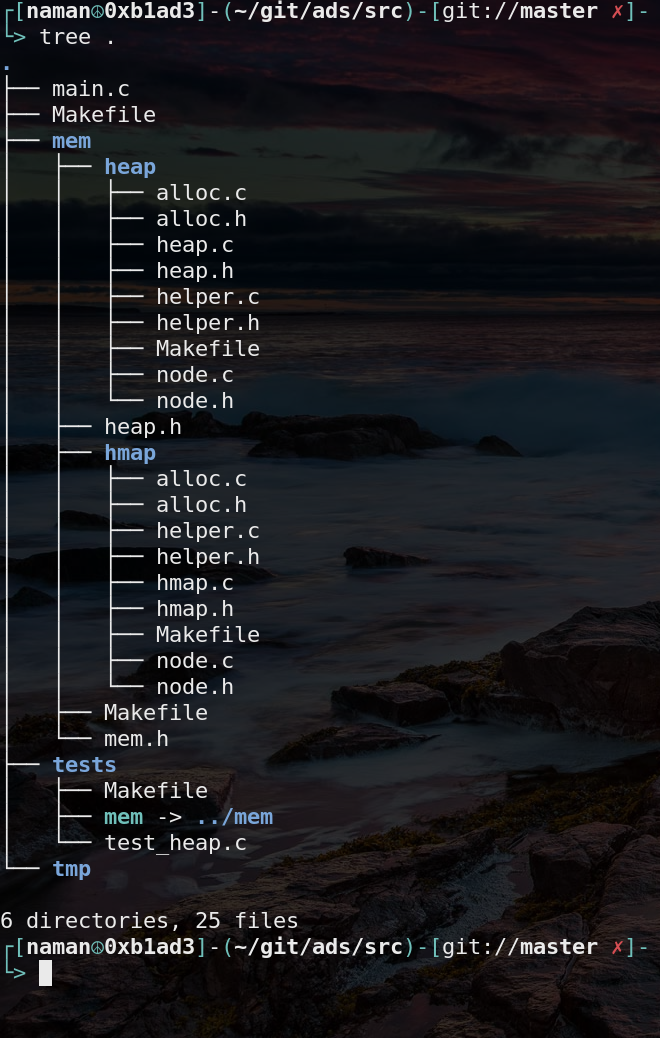
\includegraphics[width=\linewidth]{structure.png}
	  \caption{Directory Structure}
	  \label{Directory Structure}
	\end{figure}

	\begin{itemize}
		\item{\textbf{\textit{The src/ Directory}}:}
		This directory is the root of the project that contains all the sub-directories. It houses the root Makefile along with the main.c source file. The test and main binaries are produced here as a result of compilation.
		\item{\textbf{\textit{The src/mem/ Directory}}:}
		This directory houses the implementations of both hashmap and fibonacci heap. It also has the relay Makefile which further recursively calls the internal node Makefiles for the hmap/ and heap/ implementations. This has a header mem.h which is an API interface to the hmap implementation and the project as a whole. Also the header file heap.h is intended to be used internally within the hmap implementation and must not be included in caller programs.
		\item{\textbf{\textit{The src/mem/heap/ Directory}}:}
		This sub-directory resides within the src/mem/ subdirectory and houses the Fibonacci Heap implementation. It has the separated doubly linked list implementation in node.{c,h}, memory allocation and deallocation functions in alloc{c,h} as well as the heap itself in heap.{c,h} along with a helper helper{c,h}. It has the node Makefile for the heap implementation.
		\item{\textbf{\textit{The src/mem/hmap/ Directory}}:}
		This subdirectory houses the implemented hash map, implemented from scratch to encapsulate the heap implementation. This hmap basically is a hybrid of Fibonacci heap and conventional hash map so that the API user has to care about a single data structure. This is also analogous to heap implementation in the way that the directory is structured.
		\item{\textbf{\textit{The src/tests/ Directory}}:}
		This directory was initially included to implement unit tests but due to fast approaching deadline, was just shortened to a single use case test of the heap with random number generator from Libsodium. The compilation of this test thus, requires libsodium as dependency and hence is made totally independent of the real program.
	\end{itemize}
	
	\subsection{Compilation Instructions}
	The compilation requires GNU Make utility and GNU GCC compiler toolchain. It optionally requires Libsodium if tests/ is to be compiled, which is separate.
	\begin{itemize}
	\item{The main binary \textit{hashtagcounter}:}
	
		\$ make			\# To generate the binary
		
		\$ ./hashtagcounter input\_file\_location output\_file\_location		\# To run
		
	\item{The tests binary \textit{test\_out}:}
		
		\$ make tests		\# To generate tests
		
		\$ ./test\_out		\# To run the test
		
	\end{itemize}
	
	\subsection{Output Expectation}
	The Output from the main binary is expected to be a CSV file/stream depending upon if the optional output file argument is passed. The output stream/file will have the most frequent \textit{hastags} as requested in the input file for each requested output.
	
	The output from the test\_out binary is supposed to a stream of lines each with a key and its output position in descending order.
	
\section{The Code}
	Next we will gloss over the important highlights of the source code.
	\subsection{The Makefiles}
		The whole project is under the recursive compilation strategy of GNU Make utility and each subdirectory has its own makefile. There are three types of Makefiles,
		\begin{itemize}
		\item{The Root Makefile:}
		This is unique Makefile is from where the compilation process begins. It calls all the other types of Makefiles recursively from within.
		\item{The Relay Makefile:}
		This is present in the src/mem subdirectory and is just used to glue together the node Makefiles to the root one.
		\item{The Node Makefile:}
		There are three of these, \textit{viz.} src/mem/heap/Makefile, src/mem/hmap/Makefile and src/tests/Makefile. They are the ones that actually create the object binaries.
		\end{itemize}

	\subsection{The Hash Map}
	This is a pure implementation of the hash map including the hashing function in simplest of its form. This is intended to serve as the only visible entity to the end user and is designed with a first level API based structure. This encapsulates the underlying heap implementation. Some of the important functions/entities are:
	\begin{itemize}
	\item{struct hmap:}
	This is the main structure that encapsulates the hash map object and has embedded heap structure. Defined in src/mem/hmap/hmap.h
	\item{struct hmap *hmap\_init(char *, int):}
	This function initializes the hash map and is required to be called for the very first time with the very first value to be inserted. Returns the generated struct hmap. Defined in src/mem/hmap/hmap.h.
	\item{void hamp\_de\_init(struct hmap *):}
	This function deletes the whole allocated memory of the hash map.
	\item{void  hmap\_update(struct hmap *, char *, int):}
	This function accepts the new value (or an existing one) and internally decides if the a similar node exists. This accordingly calls the heap insert or increase key functions.
	\item{struct hmap\_node *hmap\_remove\_max(struct hmap *):}
	This function calls the underlying heap structure to remove the maximum value and returns it as an instance of the atomic map node, hmap\_node.
	\item{struct hmap\_node:}
	This is the atomic map instance of the hash map. It is defined in src/mem/hmap/node.h and contains the key value along with the pointer to the internal heap\_node instance.
	\item{int hash\_it(char *):}
	The hashing function used for hash map. Defined in src/mem/hmap/helper.h.
	\end{itemize}
	
	\subsection{The Fibonacci Heap}
	This is a pure implementation of the max Fibonacci heap and is housed in the subdirectory src/mem/heap. This is not intended to be used by end user and is coded as a level 2 API. It is an internal data structure for the previously defined hash map.
	\begin{itemize}
	\item{struct heap:}
	This is the main heap structure which basically contains a pointer to the current maximum node in the heap. This node is a pointer instance of struct heap\_node. Defined in src/mem/heap/heap.h
	\item{struct heap *heap\_init(int, char *):}
	This is the initialization heap function, analogous to the hmap's and returns the initialized struct heap instance.
	\item{void heap\_de\_init(struct heap *):}
	This is a de-initialization function for the heap and in turn calls the traverse function to traverse in pre order format.
	\item{void heap\_traverse(struct heap *, void (*fn)(struct heap\_node *)):}
	This function is used to traversing the heap in post order format and apply the supplied ``fn'' function prototype to each level of doubly linked list of each tree.
	\item{struct heap\_node *heap\_remove\_max(struct heap *):}
	This function removes the maximum value of from the heap and consolidates it according to the Fibonacci heap algorithm.
	\item{struct heap\_node *heap\_meld(struct heap\_node *, struct heap\_node *):}
	This melds two trees based on their keys while adjusting their degrees and returns the consolidated tree which is the root of both.
	\item{void heap\_inc\_key(struct heap *, struct heap\_node *, int):}
	This increases the key of the supplied node in the heap and adjusts the heap in accordance with the cascading child cut algorithm of the Fibonacci heap.
	\end{itemize}
	
	\subsection{The main driver}
	The main driver, in src/main.c, has two helper function, \textit{viz.}:
	\begin{itemize}
	\item{void setup(FILE **, FILE **, int, char **):}
	This function sets up the input and output file streams according to the supplied command line arguments. If no argument is provided for output file, the out file is set as stdout.
	\item{void process\_file(FILE *, FILE *):}
	This is the function that sets up the test hash map structure and reads the input file. This acts like an end used to the aforementioned API. 
	\end{itemize}

\section{Conclusion}
The programming assignment was successfully completed and was tested for 1M remove max operation on an Intel i7\-8750H Hex core processor with 16Gb virtual memory. It took about 4 Seconds and used about 8\% of the CPU. Similar and proportionally symmetrical results were obtained from testing on thunder.cise.ufl.edu server.

Further, this project can be refined via adding more decoupling to the two advanced data structures implemented upto a point where they can be used as independently with similar efficiency as being used together. The further updates will be pushed in the GitLab repository of the project:

\begin{center}
https://gitlab.com/r0ck3r008/ads
\end{center}
\end{document}